% !TeX root = ../tfg.tex
% !TeX encoding = utf8

\chapter{Análisis de datos y preprocesamiento} \label{eda}

En esta sección se presenta el análisis exploratorio de los datos disponibles en el proyecto y el preprocesamiento de los mismos. Se diferencian dos tipos de datos principales: los volúmenes de imagen originales en tipo DICOM y los datos clínicos tabulares. El objetivo de este análisis es entender la estructura, características y potenciales problemas de los datos antes de diseñar el preprocesamiento y los modelos.

% -----------------------------
\section{Análisis de datos}
Empezamos con el análisis de los volúmenes de imagen en formato DICOM, que constituyen la base del dataset.
% -----------------------------
\subsection{Análisis de datos de volúmenes DICOM}
El segundo componente del dataset corresponde a los volúmenes de imagen en formato DICOM. Para su análisis, se recorrieron de forma recursiva las carpetas anonimizadas para contabilizar los archivos correspondientes a cada paciente y extraer características como el número de slices (profundidad del volumen) y la resolución axial (Height y Width).

Para empezar, se generó un histograma para visualizar la distribución del número de slices por volumen. La distribución es claramente asimétrica y presenta un sesgo hacia la derecha, con un pico principal entre aproximadamente 200 y 300 cortes por paciente. Sin embargo, existen casos con más de 900 slices, considerados outliers.


\begin{figure}[!htbp]
    \centering
    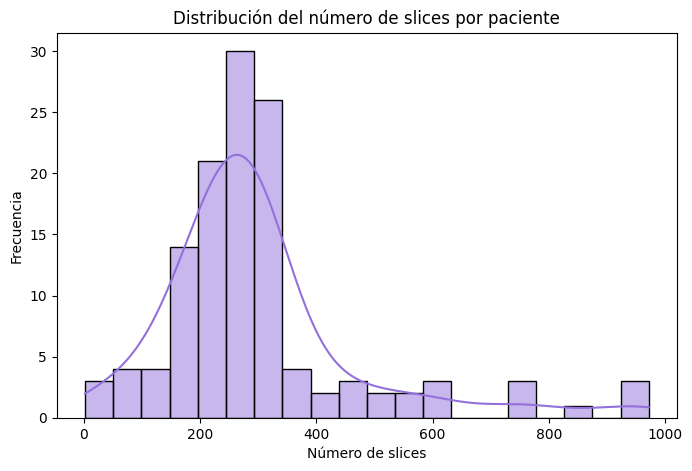
\includegraphics[width=0.7\textwidth]{img/histograma_dist_slices_x_paciente.png}
    \caption{Distribución del número de slices por paciente.}
    \label{fig:distribucion_slices}
\end{figure}

La alta variabilidad mostrada en la Figura \ref{fig:distribucion_slices} en la dimensión axial es importante porque, en modelos de redes convolucionales 3D, la entrada debe tener un tamaño fijo en todas sus dimensiones. Por ello, será necesario aplicar técnicas de preprocesamiento para normalizar este eje, como el recorte central de slices o la interpolación lineal para aumentar el número de cortes en volúmenes más pequeños.


En cuanto a las dimensiones de cada corte (height y width), se han encontrado dos resoluciones:

\begin{itemize}
    \item \textbf{512x512}: presente en 70 volúmenes.
    \item \textbf{768x768}: presente en 55 volúmenes.
\end{itemize}

Esta relativa homogeneidad facilitará el preprocesamiento, permitiendo reescalar todas las imágenes a un tamaño fijo común para garantizar consistencia en los datos de entrada del modelo.


\subsection{Análisis exploratorio de datos clínicos}
El conjunto de datos clínicos contiene información de 125 pacientes, cada uno identificado mediante un código único. En la recopilación original de los datos médicos se incluían las siguientes variables: Identificador del paciente, Sexo, Edad, Tipo de cáncer, Complicación, Tipo de complicación, Factor de riesgo, Patología pulmonar, Extensión al diagnóstico, TC (máquina en la que se realiza la prueba), Extensión a los 5 años y Mutación.

Sin embargo, muchas de estas variables se conocen únicamente tras la biopsia, por lo que su inclusión en el entrenamiento del modelo introduciría un sesgo de información. Por este motivo, se han eliminado las variables \textit{Extensión al diagnóstico}, \textit{TC}, \textit{Extensión a los 5 años} y \textit{Mutación}. Además, aunque el \textit{Tipo de cáncer} se elimina en el preprocesamiento, se ha mantenido su análisis descriptivo dado que proporciona contexto clínico relevante.

Tras este filtrado inicial, las variables de interés para el análisis exploratorio son:

\begin{itemize}
    \item \textbf{Identificador del paciente}: código único para trazabilidad (no usado en entrenamiento).
    \item \textbf{Sexo}: variable categórica binaria (Hombre/Mujer). Se observa un ligero desbalanceo hacia la categoría masculina.
    \item \textbf{Edad}: variable numérica entera. La distribución está centrada en el rango de 65-70 años, destacando la predominancia de pacientes de edad avanzada.
    \item \textbf{Complicación}: variable objetivo binaria (Sí/No). Presenta un leve desbalanceo hacia la ausencia de complicación.
    \item \textbf{Tipo de complicación}: variable categórica multietiqueta (solo para casos positivos).
    \item \textbf{Factor de riesgo}: variable de texto con potencial multietiqueta.
    \item \textbf{Patología pulmonar}: condiciones respiratorias previas. Variable de texto también multietiqueta.
    \item \textbf{Tipo de cáncer}: aunque se elimina en preprocesamiento, se analiza aquí por ser el cáncer de pulmón el principal problema de estudio.
\end{itemize}

Antes de realizar el análisis estadístico, se llevó a cabo un proceso exhaustivo de limpieza, corrigiendo errores de ortografía, unificando conceptos médicos sinónimos y eliminando inconsistencias. Tras la limpieza, se verificó la ausencia de valores nulos.


\begin{figure}[!htbp]
    \centering
    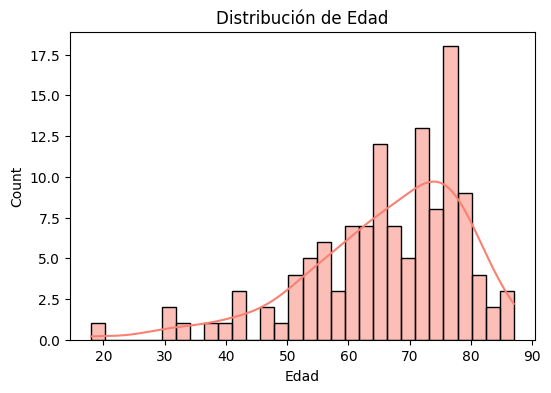
\includegraphics[width=0.65\textwidth]{img/histograma_dist_edad.png}
    \caption{Distribución de la edad de los pacientes.}
    \label{fig:distribucion_edad}
\end{figure}

En el histograma de edad de la Figura \ref{fig:distribucion_edad} se aprecia cómo la mayoría de los pacientes se agrupa en la franja de 65 a 80 años, con muy pocos casos por debajo de los 30 años. Esto refleja que se trata de una población mayor, aspecto importante para la interpretación clínica y la generalización del modelo.


\begin{figure}[!htbp]
    \centering
    \begin{minipage}[b]{0.45\textwidth}
        \centering
        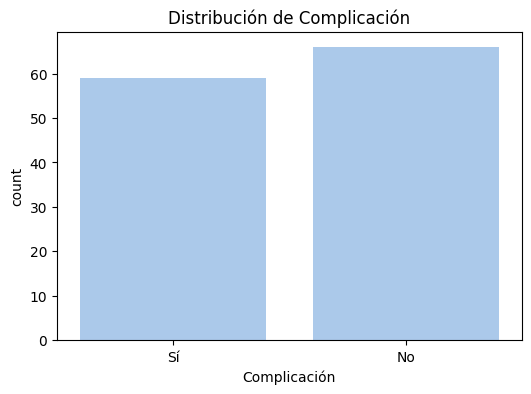
\includegraphics[width=\textwidth]{img/histograma_dist_complicacion.png}
        \caption{Distribución de la variable Complicación (Sí / No).}
        \label{fig:distribucion_complicacion}
    \end{minipage}
    \hspace{0.05\textwidth}
    \begin{minipage}[b]{0.45\textwidth}
        \centering
        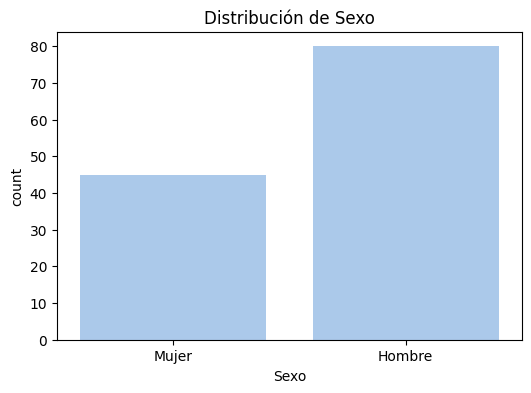
\includegraphics[width=\textwidth]{img/histograma_dist_sexo.png}
        \caption{Distribución de la variable Sexo (Hombre / Mujer).}
        \label{fig:distribucion_sexo}
    \end{minipage}
\end{figure}

La Figura \ref{fig:distribucion_complicacion} muestra que la variable \textit{Complicación} presenta un leve desbalanceo hacia los casos sin complicación, mientras que la Figura \ref{fig:distribucion_sexo} muestra que la variable \textit{Sexo} tiene un predominio masculino. Cabe destacar que el tema del desbalanceo en la variable \textit{Complicación} se estudió especialmente durante las primeras fases del proyecto, ya que con los datos disponibles hasta ese momento el desbalanceo era considerable. Sin embargo, con la llegada de nuevos lotes y la base de datos completa, dicho desbalanceo se redujo significativamente, por lo que no fue necesario aplicar técnicas específicas en las fases finales. Por su parte, el desbalanceo en la variable \textit{Sexo} no ha sido tratado de forma específica.

Como parte del análisis exploratorio, se estudió la distribución de la Figura \ref{fig:distribucion_tipo_cancer} del \textit{Tipo de cáncer}, aunque esta variable se eliminará en el entrenamiento. 

\begin{figure}[!htbp]
    \centering
    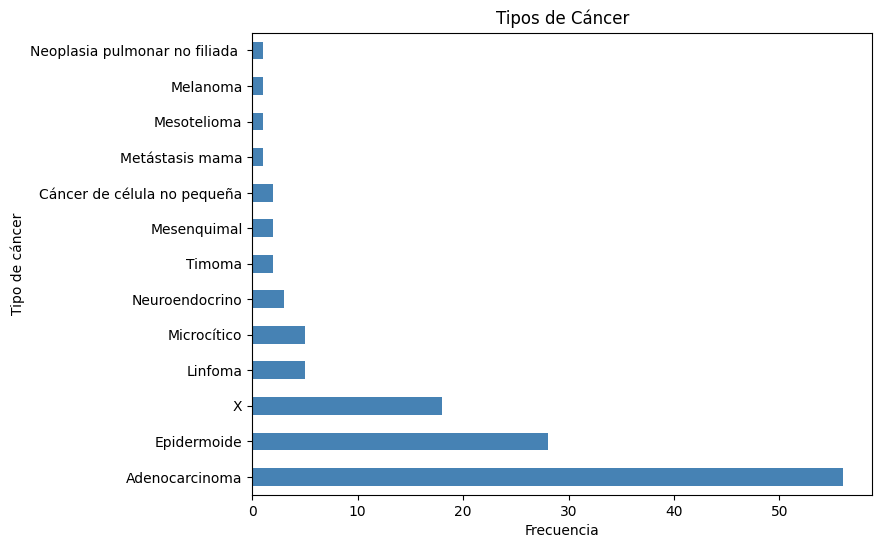
\includegraphics[width=1\textwidth]{img/barras_tipo_cancer.png}
    \caption{Frecuencia de categorías en Tipo de cáncer.}
    \label{fig:distribucion_tipo_cancer}
\end{figure}
 

Para las variables multietiqueta como \textit{Tipo de complicación}, \textit{Factor de riesgo} y \textit{Patología pulmonar} (Figuras  \ref{fig:distribucion_tipo_complicacion}, \ref{fig:distribucion_patologia_pulmonar} y \ref{fig:distribucion_factor_riesgo} respectivamente), se analizaron sus distribuciones para entender la diversidad de categorías presentes en el dataset. 


\begin{figure}[!htbp]
    \centering
    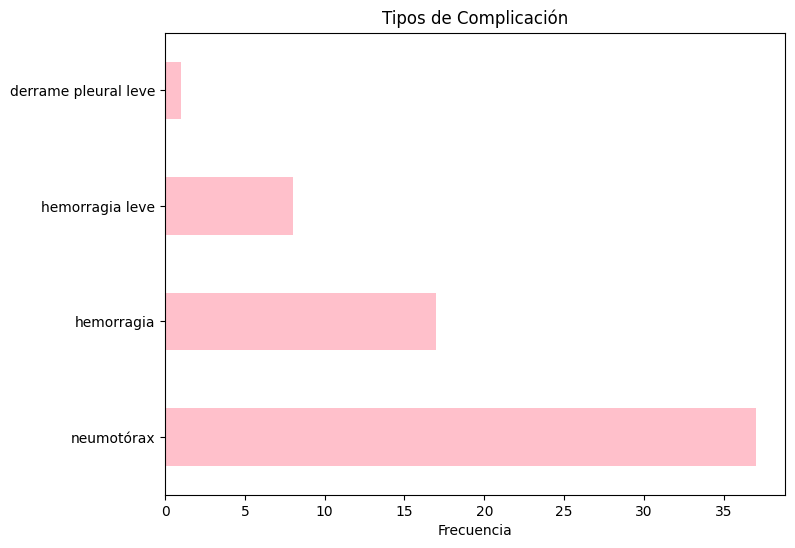
\includegraphics[width=1\textwidth]{img/barras_tipo_complicacion.png}
    \caption{Frecuencia de categorías en Tipo de complicación.}
    \label{fig:distribucion_tipo_complicacion}
\end{figure}


\begin{figure}[!htbp]
    \centering
    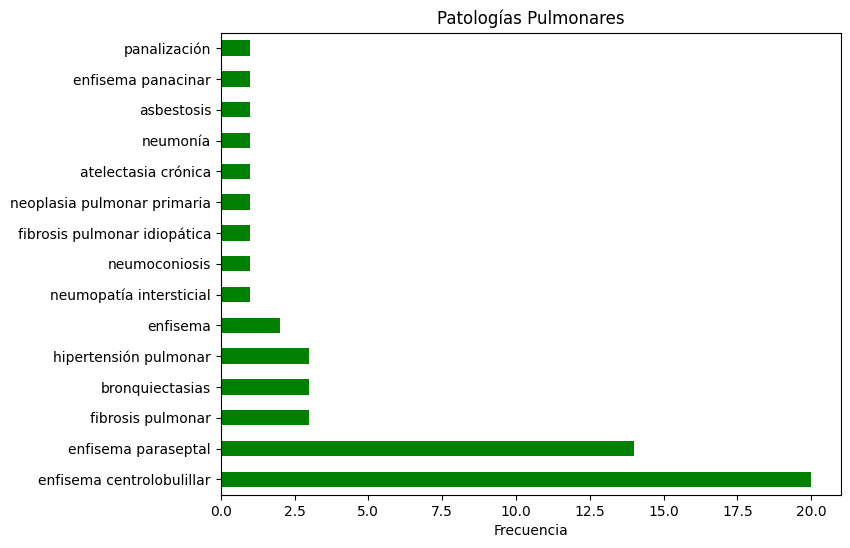
\includegraphics[width=1\textwidth]{img/barras_patologia_pulmonar.png}
    \caption{Frecuencia de categorías en Patología pulmonar.}
    \label{fig:distribucion_patologia_pulmonar}
\end{figure}


\begin{figure}[!htbp]
    \centering
    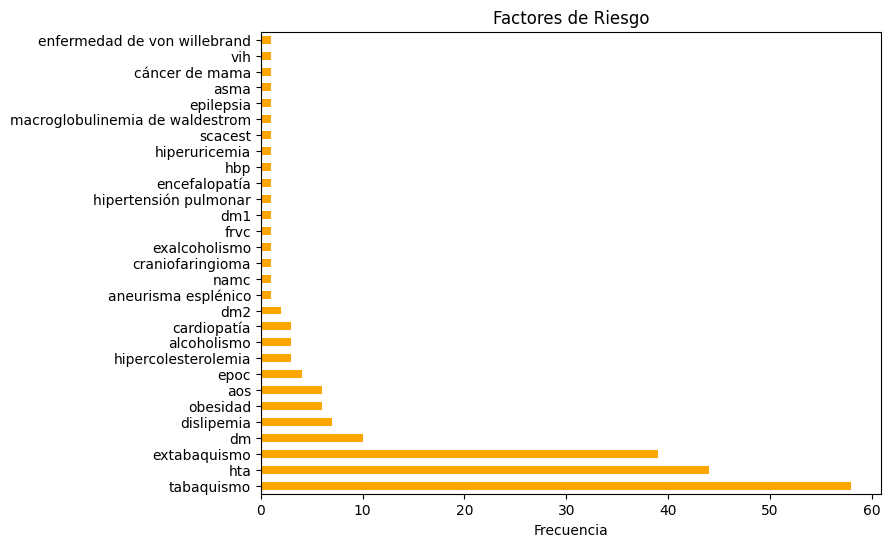
\includegraphics[width=1\textwidth]{img/barras_factor_riesgo.png}
    \caption{Frecuencia de categorías en Factor de riesgo.}
    \label{fig:distribucion_factor_riesgo}
\end{figure}


El análisis de estas variables evidencia una considerable diversidad y riqueza semántica, lo que justifica la necesidad de aplicar un preprocesamiento multietiqueta para transformarlas en variables utilizables en un modelo de aprendizaje automático.

En conclusión, el análisis de los datos clínicos confirma la ausencia de valores nulos, un ligero desbalanceo de clases y una población predominantemente mayor.




% ----------------------------------------------------------------------

\section{Preprocesamiento de los datos} \label{sec:preprocesamiento}

Tras el análisis exploratorio, se realizó el preprocesamiento en Python adaptado a las características del dataset, con el objetivo de estandarizar el formato de entrada y reducir la variabilidad innecesaria que pudiera afectar al entrenamiento de modelos. Este preprocesamiento abarca tanto los datos clínicos tabulares como los volúmenes de imagen médica en formato DICOM, asegurando una preparación coherente y homogénea de todas las fuentes de datos.

\subsection{Preprocesamiento de datos de volúmenes DICOM}

\subsubsection{Introducción a MONAI para el modelado de imágenes médicas}

Para los volúmenes DICOM se utilizó principalmente MONAI, una biblioteca especializada en el procesamiento y modelado de imágenes médicas. Se implementó un preprocesamiento modular basado en MONAI, complementado con transformaciones personalizadas adaptadas al dominio clínico. Los pipelines se construyeron de forma modular y configurable, definiendo versiones para entrenamiento y validación. 

\subsubsection{Igualación de tamaños de imágenes}

Para abordar la alta variabilidad en la forma de los volúmenes (con diferente número de cortes y resoluciones como 512x512 o 768x768), se empleó una interpolación trilineal para normalizar todos los volúmenes a un tamaño objetivo uniforme. Esto asegura entradas de tamaño constante, crucial para el entrenamiento de redes convolucionales 3D. La interpolación trilineal preserva la continuidad espacial y anatómica, manteniendo la coherencia del volumen.

Se exploraron diferentes tamaños para estos volúmenes, evaluando su impacto en el entrenamiento. Inicialmente, se utilizaron resoluciones grandes como (256,512,512) o (128,256,256), con el objetivo de preservar el mayor detalle posible. Sin embargo, en los análisis con técnicas de explicabilidad se observó que el modelo a menudo se fijaba en regiones irrelevantes, posiblemente debido al exceso de información redundante. Por ello, se ensayaron también resoluciones más reducidas, como (128,128,128), (64,64,64) e incluso (28,28,28). Estos tamaños más compactos ayudaban a forzar al modelo a centrarse en patrones globales más relevantes y a mitigar el sobreajuste a detalles poco útiles. No obstante, las resoluciones más pequeñas como (28,28,28) se descartaron por perder demasiado detalle anatómico. Fueron inicialmente utilizadas por similitud a datasets para preentrenamiento, ya que utilizaban imágenes médicas de ese tamaño. 

\subsubsection{Data augmentation}

Se han probado diferentes tipos de preprocesamiento, uno de ellos incluye también transformaciones de data augmentation como \texttt{RandAffine}, que aplica rotaciones, escalados y traslaciones aleatorias, simulando variabilidad anatómica y de posicionamiento del paciente. Estas transformaciones son leves para no distorsionar demasiado las imágenes, mejorando así la capacidad de generalización del modelo al exponerlo a ligeras variaciones geométricas de los datos de entrenamiento.

\subsubsection{Ventanas de Hounsfield}

En TC, el valor de cada voxel en la imagen reconstruida refleja el coeficiente de atenuación lineal del haz de rayos X al atravesar el tejido correspondiente \parencite{calzado2010tomografia}. Para estandarizar su interpretación, estos coeficientes se transforman en la escala de \textit{unidades Hounsfield (HU)}, que usa el agua a temperatura ambiente como referencia de 0 HU y el aire como -1000 HU. Esta transformación se define mediante la fórmula:

\[
HU_{mat} = \frac{\mu_{mat} - \mu_{agua}}{\mu_{agua}} \times 1000
\]

donde $\mu_{mat}$ es el coeficiente de atenuación lineal del material o tejido y $\mu_{agua}$ el del agua. Cada incremento de 1 HU corresponde a un cambio del 0,1\% en la atenuación relativa al agua.  

La escala Hounsfield abarca un rango amplio de valores: el aire se define como -1000 HU (pues apenas atenúa), el agua como 0 HU, y el tejido adiposo suele encontrarse entre -100 y -80 HU. El parénquima pulmonar se sitúa aproximadamente entre -950 y -600 HU, mientras que la mayoría de tejidos blandos se representan con valores de 20 a 70 HU. Por su parte, el hueso compacto puede superar los +1000 HU, reflejando su elevada densidad.

En la adquisición de imágenes, los escáneres suelen almacenar estos valores con una profundidad mínima de 12 bits, cubriendo un rango aproximado de -1024 a +3071 HU, suficiente para la mayoría de tejidos clínicos. Sin embargo, algunas aplicaciones utilizan 14 bits para ampliar esta escala hasta más de +15.000 HU, permitiendo representar materiales de alta densidad, como implantes metálicos, stents o prótesis ortopédicas, sin saturación en la imagen.

Para visualizar estas imágenes en monitores médicos, que suelen limitarse a 8 o 12 bits (256 o 4096 niveles de gris), se utiliza el concepto de \textit{ventana de visualización}. Esta técnica permite ajustar el rango de HU mostrado para optimizar la visualización de diferentes tipos de tejidos. Está caracterizada por dos parámetros fundamentales:

\begin{itemize}
    \item \textbf{Window Level (WL)}: nivel central de la ventana, que define qué valor de HU aparecerá como gris medio.
    \item \textbf{Window Width (WW)}: ancho de la ventana, que determina el rango total de HU representado desde negro hasta blanco.
\end{itemize}

Al ajustar WL y WW, los radiólogos pueden resaltar estructuras específicas. Por ejemplo, en el análisis del parénquima pulmonar se suelen usar ventanas con WL $\approx$ -600 HU y WW $\approx$ 1500 HU para resaltar lesiones como nódulos, consolidaciones o enfisema (veáse la Figura \ref{fig:hu-ejemplo}). Para tejidos blandos del mediastino o abdomen se usan combinaciones distintas de WL y WW para optimizar el contraste en esas estructuras.

Sin embargo, los valores de HU pueden verse afectados por diversos factores técnicos: la tensión del tubo de rayos X (kVp) influye en la atenuación relativa, sobre todo en materiales de alto número atómico como el hueso (calcio) o el contraste yodado; además, el filtro de reconstrucción, el campo de visión (FOV), la posición del objeto escaneado o incluso artefactos pueden introducir variaciones en los valores registrados. A esto se suman posibles desviaciones sistemáticas entre equipos diferentes o la deriva temporal de un mismo escáner. Por ello, en estudios multicéntricos o longitudinales se requiere especial cuidado en la calibración y armonización de los valores HU para garantizar la comparabilidad cuantitativa.

Para este proyecto, se han diseñado transformaciones específicas en el pipeline de MONAI que aplican de forma sistemática y reproducible las ventanas clínicas relevantes. Estas transformaciones recortan los valores de HU a rangos clínicamente significativos y los normalizan al intervalo [0,1], facilitando el aprendizaje del modelo al centrarse en la información más útil. En concreto, se implementaron dos enfoques principales:

\begin{itemize}
    \item \textbf{Windowingd}: aplica una única ventana (por ejemplo, la ventana pulmonar), generando un canal de entrada optimizado para resaltar el parénquima y sus lesiones.
    \item \textbf{MultiWindowingd}: aplica varias ventanas (pulmón, mediastino, consolidación) y apila los resultados como canales independientes, creando una representación multicanal que enriquece la información anatómica y patológica disponible para el modelo.
\end{itemize}

\begin{figure}[!htbp]
    \centering
    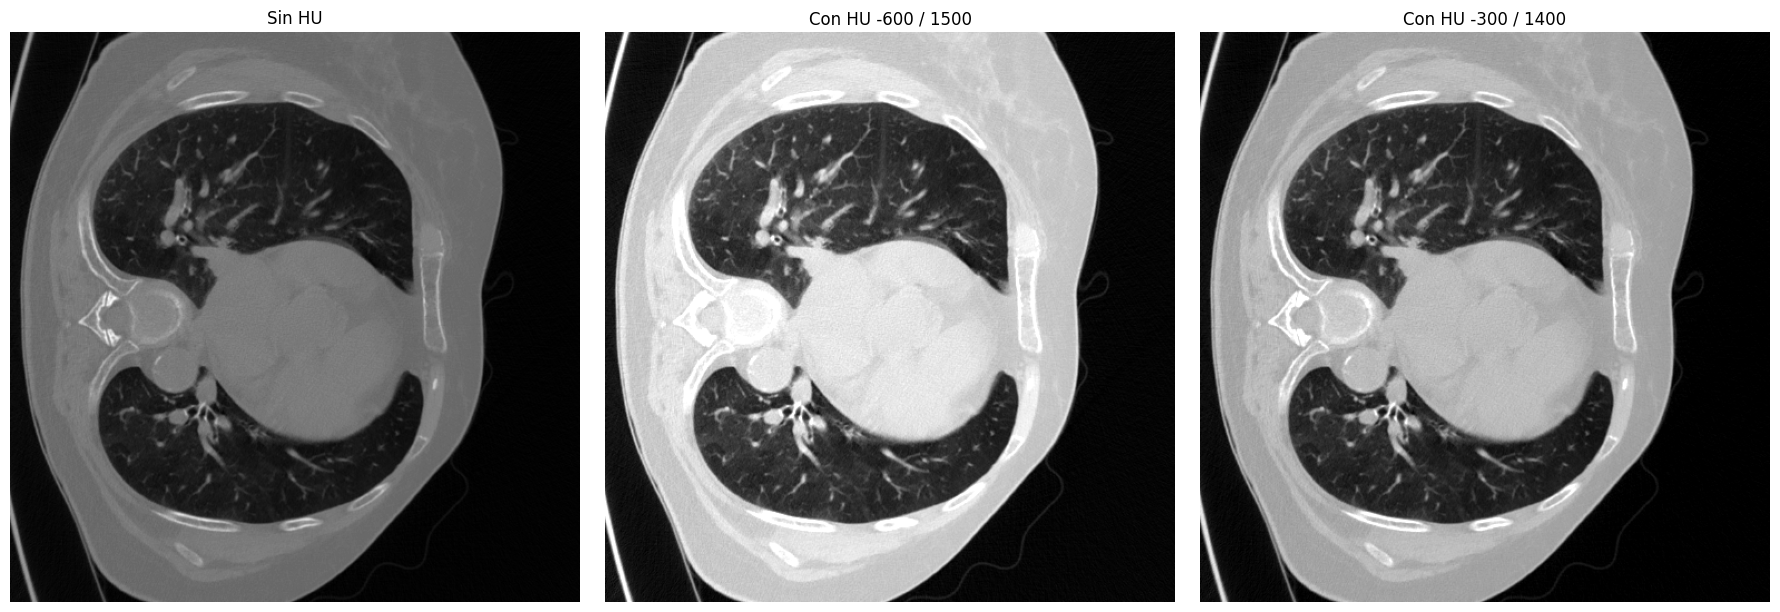
\includegraphics[width=1\textwidth]{img/hu_ejemplos.png}
    \caption{Comparación de la misma imagen axial de TC preprocesada con diferentes configuraciones de ventana HU: sin ventana, con ventana centrada en -600 HU (ancho 1500) y con ventana centrada en -300 HU (ancho 1400). Se observa la mejora de contraste en el parénquima pulmonar tras aplicar el recorte de intensidades. Elaboración propia.}
    \label{fig:hu-ejemplo}
\end{figure}

Estas estrategias imitan el proceso diagnóstico clínico, donde el radiólogo ajusta las ventanas para identificar con mayor claridad las estructuras relevantes, mejorando así la interpretabilidad y el rendimiento del modelo en tareas de clasificación o segmentación.

\subsubsection{Segmentación}

Durante las primeras fases de experimentación se utilizaron los volúmenes 3D originales de TC sin ningún tipo de segmentación previa. Sin embargo, al aplicar técnicas de explicabilidad y analizar los mapas de activación de los modelos, se observó que en numerosas ocasiones el modelo se fijaba en regiones externas al pulmón. Esto introducía un sesgo importante, ya que la red podía aprender patrones irrelevantes y no relacionados con las complicaciones pulmonares que se pretendían predecir.

Para mitigar este problema y forzar al modelo a centrarse únicamente en la región anatómica de interés, se incorporó un paso de \textit{segmentación pulmonar}. La segmentación permite aislar el volumen pulmonar, eliminando estructuras irrelevantes y reduciendo el ruido de fondo. De esta forma, se mejora la capacidad del modelo para aprender patrones verdaderamente discriminativos y clínicamente relevantes.

La generación de máscaras de pulmón se realizó de forma completamente automatizada utilizando la herramienta \texttt{TotalSegmentator} \parencite{wasserthal2023totalsegmentator}, una solución basada en aprendizaje profundo que ofrece modelos preentrenados para segmentación médica. En este caso, se empleó la tarea específica de segmentación pulmonar, que produce máscaras binarias indicando únicamente la localización de los pulmones en cada volumen. Se pueden observar dos ejemplos de esta segmentación (uno en 2D y otro en 3D) en las Figura \ref{fig:ejemplo-segmentacion} y \ref{fig:ejemplo-segmentacion3D}. Los datos DICOM originales se convirtieron previamente al formato NIfTI (.nii) para compatibilidad con el modelo, y las máscaras generadas se almacenaron con nomenclatura estandarizada para su posterior uso.

Una vez generadas las máscaras pulmonares, se integraron en el flujo de preprocesamiento mediante la transformación \texttt{CombineMaskAndImage}. Esta operación permite combinar la imagen original y su máscara segmentada de dos formas principales: 
\begin{itemize}
    \item \textbf{stack}: apilando la máscara como un canal adicional para que el modelo disponga explícitamente de la información sobre la localización pulmonar.
    \item \textbf{mask\_zero\_out}: enmascarando las regiones externas al pulmón con valores HU muy bajos, forzando al modelo a ignorar información irrelevante.
\end{itemize}
Esta flexibilidad permite experimentar con diferentes enfoques, desde obligar a la red a centrarse solo en el pulmón.

\subsection{Preprocesamiento de datos clínicos tabulares}

Para los datos clínicos tabulares se utilizó la biblioteca scikit-learn de Python. El proceso comenzó con la eliminación de columnas que contenían información únicamente disponible \textit{a posteriori}, como el \textit{Tipo de cáncer}, evitando así la introducción de fugas de información en el entrenamiento. Posteriormente, se abordó el tratamiento de variables multietiqueta, como \textit{Factor de riesgo} y \textit{Patología pulmonar}. Estas columnas incluían múltiples etiquetas separadas por comas, lo que requería una limpieza para unificar nomenclaturas y corregir inconsistencias. Además, se reemplazaron valores nulos o el marcador especial \texttt{X} por etiquetas explícitas como \textit{Sin complicación} o \textit{Sin factor de riesgo}. Para transformar estos datos en un formato apto para modelos de aprendizaje automático, se aplicó un esquema de binarización multietiqueta mediante \texttt{MultiLabelBinarizer}, generando variables one-hot que representan la presencia o ausencia de cada etiqueta.

La variable \textit{Edad} fue normalizada en el rango [0,1] utilizando \texttt{MinMaxScaler}, para evitar problemas de escala y facilitar el aprendizaje del modelo. Además, la variable objetivo \textit{Complicación}, originalmente categórica con valores \textit{Sí o No}, se transformó en binaria asignando \textit{1 o 0} respectivamente. Como resultado final, se obtuvo un conjunto de datos tabular limpio y consistente, con variables numéricas y binarias, libre de valores nulos y con un formato adecuado para entrenamiento, que se almacenó en formato CSV para uso posterior.

\begin{figure}[!htbp]
    \centering
    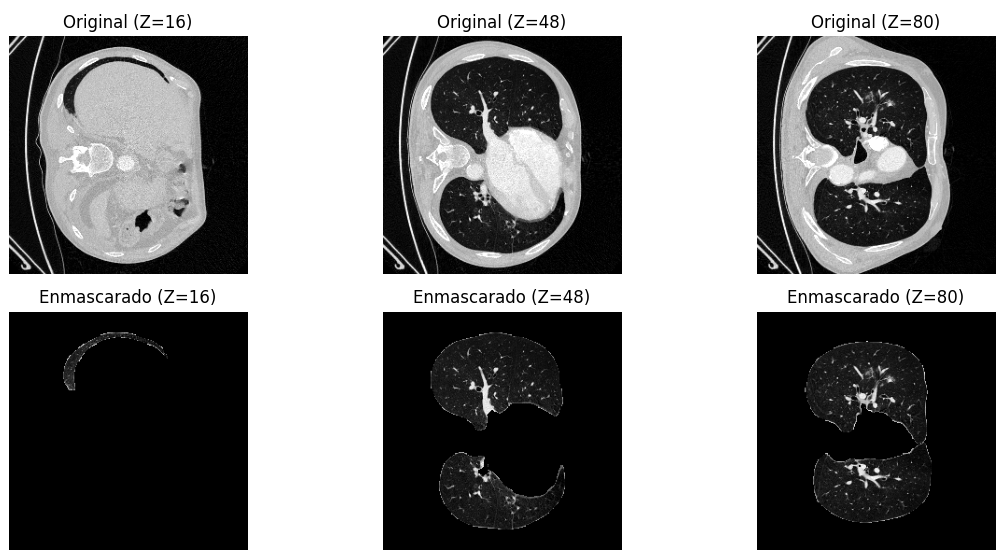
\includegraphics[width=1\textwidth]{img/ejemplo_segmentacion.png}
    \caption{Ejemplo de un volumen antes y después de la segmentación. Elaboración propia.}
    \label{fig:ejemplo-segmentacion}
\end{figure}

\begin{figure}[!htbp]
    \centering
    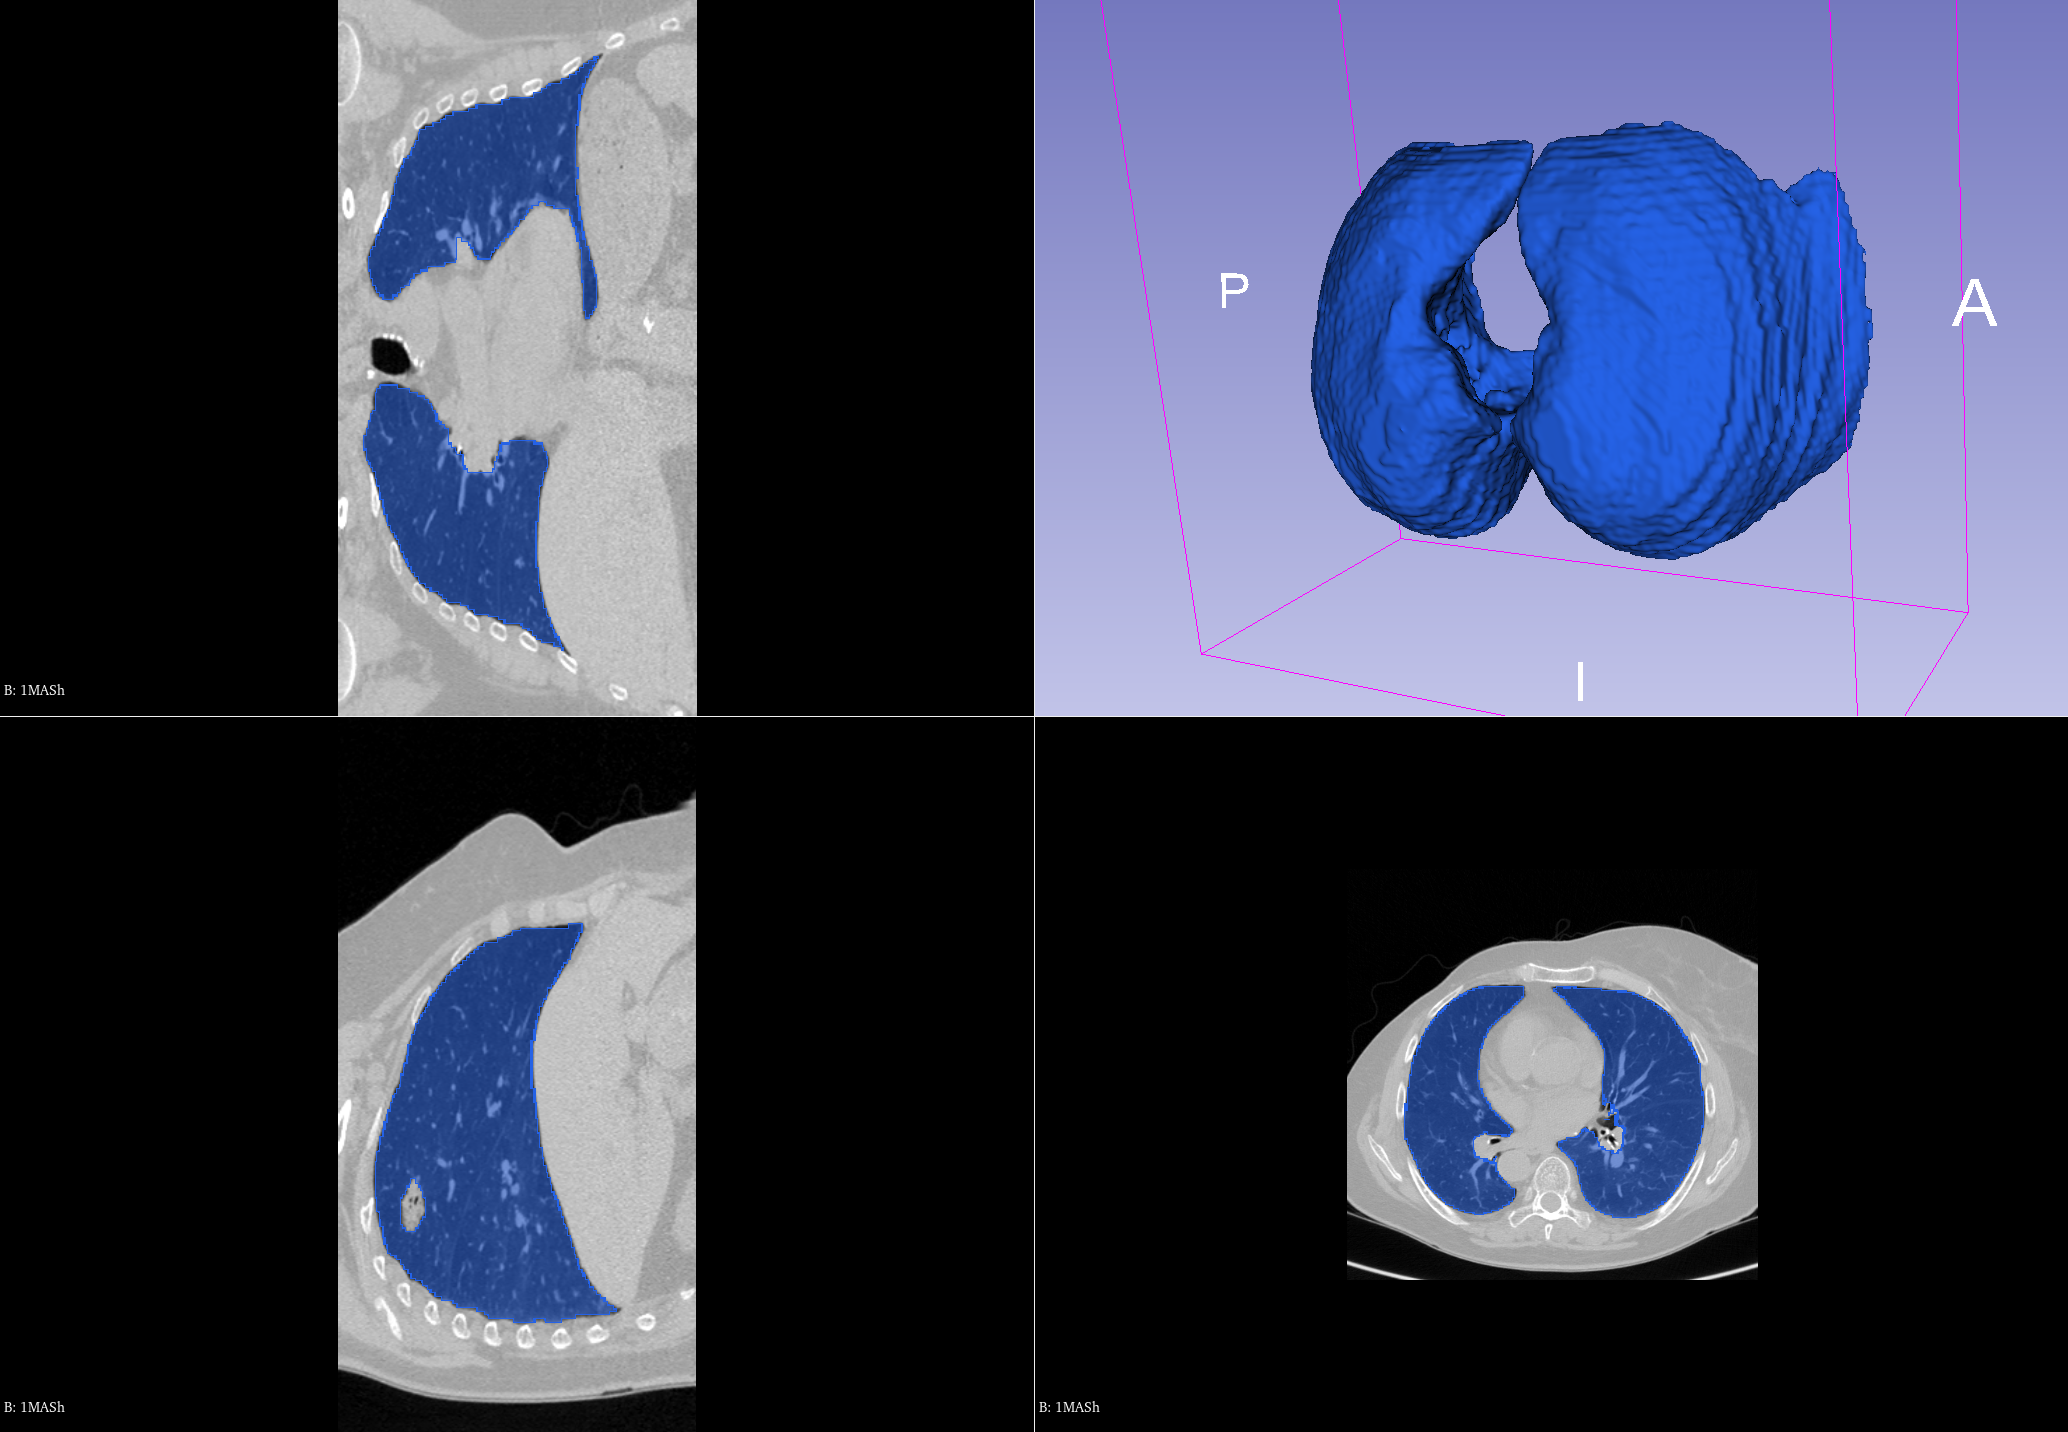
\includegraphics[width=1\textwidth]{img/segmentacion3D.png}
    \caption{Ejemplo de segmentación en 3D y en los 3 planos anatómicos en 2D. Elaboración propia realizada con 3D Slicer.}
    \label{fig:ejemplo-segmentacion3D}
\end{figure}


\endinput
%--------------------------------------------------------------------
% FIN DEL CAPÍTULO. 
%--------------------------------------------------------------------
